\documentclass[10pt]{beamer}

\usetheme[progressbar=frametitle]{metropolis}
\usepackage{appendixnumberbeamer}

\usepackage{booktabs}
\usepackage[scale=2]{ccicons}

\usepackage{pgfplots}
\usepgfplotslibrary{dateplot}

\usepackage{xspace}
\newcommand{\themename}{\textbf{\textsc{metropolis}}\xspace}

\title{Redes definidas por software}
\subtitle{Redes de computadoras 2019-1}
% \date{\today}
\date{}
\author{Arteaga Hernández Alejandro}
\institute{Universidad Autónoma de México}
% \titlegraphic{\hfill\includegraphics[height=1.5cm]{logo.pdf}}

\begin{document}

\maketitle



\section{Introducción}

\begin{frame}[fragile]{Introducción}

Las redes definidas por software (SDN) conocidas también como
redes programables y automatizadas, se presentan como una
propuesta que brinda mayor velocidad, infraestructura ágil y
mejores costos en plataformas cloud IT, urge responder al
dinamismo de las aplicaciones que requiere el usuario.\\
• ¿Cuáles son los desafíos que enfrentan las empresas al
implementar las SDN? 
\end{frame}


\begin{frame}[fragile]{Antecedentes}
Las redes no han cambiado hace unos 30 años a diferencia
de los programas, estamos enfrentando un cambio de
paradigma al cual debemos adecuarnos.
• El desarrollo de las SDN se iniciaron a partir de 1990, donde
se incluye funciones programables en la red, en el 2001-
2007, se separó el plano de control y de datos mejorando
con esta innovación, a partir del 2007-2010, se implementa
los API OpenFlow, se presenta como una interfaz abierta,
presenta diversas maneras la separación del plano de control
y de datos para que sea escalable, práctica donde
virtualización jugó un rol importante en esta evolución de
SDN.
\end{frame}

\section{¿Por qué surgen?}

\begin{frame}{¿Por qué?}
\begin{itemize}
\item Surge debido a que los data center no pueden responder a patrones de trafico impredecibles y a los picos de demanda.
\item Se tendría dos alternativas: escalar a una red mas cara empleando mas tiempo de configuración o adecuarse a una red dinámica.
\item SDN es adecuado para clientes que requieren cambios rápidos y en corto plazo.
\item Actualmente los clientes usan redes sociales, tienen una gran demanda o requieren cambios repentinos, por ejemplo trabajar sobre tráfico geográfico.
\item Desarrollo de dispositivos móviles.
\item Virtualización de dispositivos de red.
\item Servicios en la nube.
\end{itemize}
\end{frame}

\begin{frame}{Características}
\begin{itemize}
\item Infraestructura programable.
\item Administración centralizada.
\item Abstracción de la red: separa el plano de control del plano de datos.
\item Flexibilidad y actualización en tiempo real.
\item Automatización.
\item Open source y neutralidad del fabricante.
\end{itemize}
\end{frame}


\begin{frame}{Figura}
    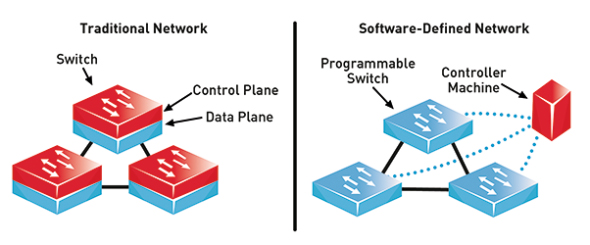
\includegraphics[scale=0.5]{sdn.jpg}
\end{frame}

\section{¡Gracias!}


\end{document}
